\chapter{Модель АНПА}
\section{Описание модели АНПА} \label{sec:model_anpa}
\subsection{Декомпозиция}

Исследуемый объект контроля представляет собой АНПА, предназначенный для поиска скоплений планктона,
рыбных косяков или китов под водой путем испускания специализированной зондирующей посылки и ее анализа.
АНПА заключен в металлический корпус, внутри которого располагаются составные части.
В данной модели предполагается, что прибор управления является центральным управляющим узлом изделия,
на который возложены все функции принятия решений.

Для проверки объекта контроля АНПА необходима система контроля.
Создание и отладка СК сопряжена со следующими факторами.
\begin{enumerate}
    \item Дороговизна и труднодоступность достаточного количества статистического материала
    натурных испытаний для отладки алгоритмов ПО СК экономически нецелесообразна, так же связана с риском для жизни испытующих.
    \item ОК находится на этапе проектирования.
    \item Отсутствует возможность непосредственного подключения к ОК.
    \item Проверка граничных значений алгоритмов ОК, ведущих к разрушению ОК недопустима.
\end{enumerate}
На этапах создания и отладки ПО СК необходимо иметь возможность проверки
функционирования алгоритмов проверки без прямого подключения к ОК.
Этого можно достичь путем создания имитатора АНПА ОК на базе ПЛК и системы аналогово-дискретных
модулей ввода-вывода.
В текущих проектах стоимость подобного набора начинается от 500~тысяч рублей,
при этом следующие риски присущи этому подходу:
\begin{itemize}
    \item увеличение накладных расходов (добавочная стоимость);
    \item увеличение сроков разработки, так как невозможно провести проверки в полном объеме до 
        создания, сборки и отладки имитатора на базе ПЛК;
    \item риски, связанные со сроками поставки комплектующих имитатора на базе ПЛК.
\end{itemize}
Выбирая этот подход, возникает следующая проблема. При начале работы над новым проектом объекта контроля
использовать уже имеющиеся комплектующие для создания другого имитатора на базе ПЛК или же заказать новые.

При выборе первого сценария возможны следующие осложнения.
\begin{enumerate}
    \item Придется частично или полностью разобрать имеющийся имитатор, тем самым при возникновении 
        осложнений с предыдущим ОК придется заново собирать его.
    \item Использовать систему тумблеров для коммутации электрических сигналов,
        увеличивая сложность аппаратной составляющей имитатора на базе ПЛК.
    \item Использовать программные средства (if-else ветвления), что увеличит сложность программы имитатора.
    \item Так же нельзя исключать пресловутый человеческий фактор.
\end{enumerate}

Тем не менее, прежде чем приступать к разработке ПО системы контроля необходимо провести анализ СЧ АНПА.
Составные части рассматриваемой модели АНПА показаны на рисунке \ref{fig:model_anpa} и в таблице \ref{tbl:model_anpa_objects}.
\begin{center}
    \begin{figure}[hb!]
        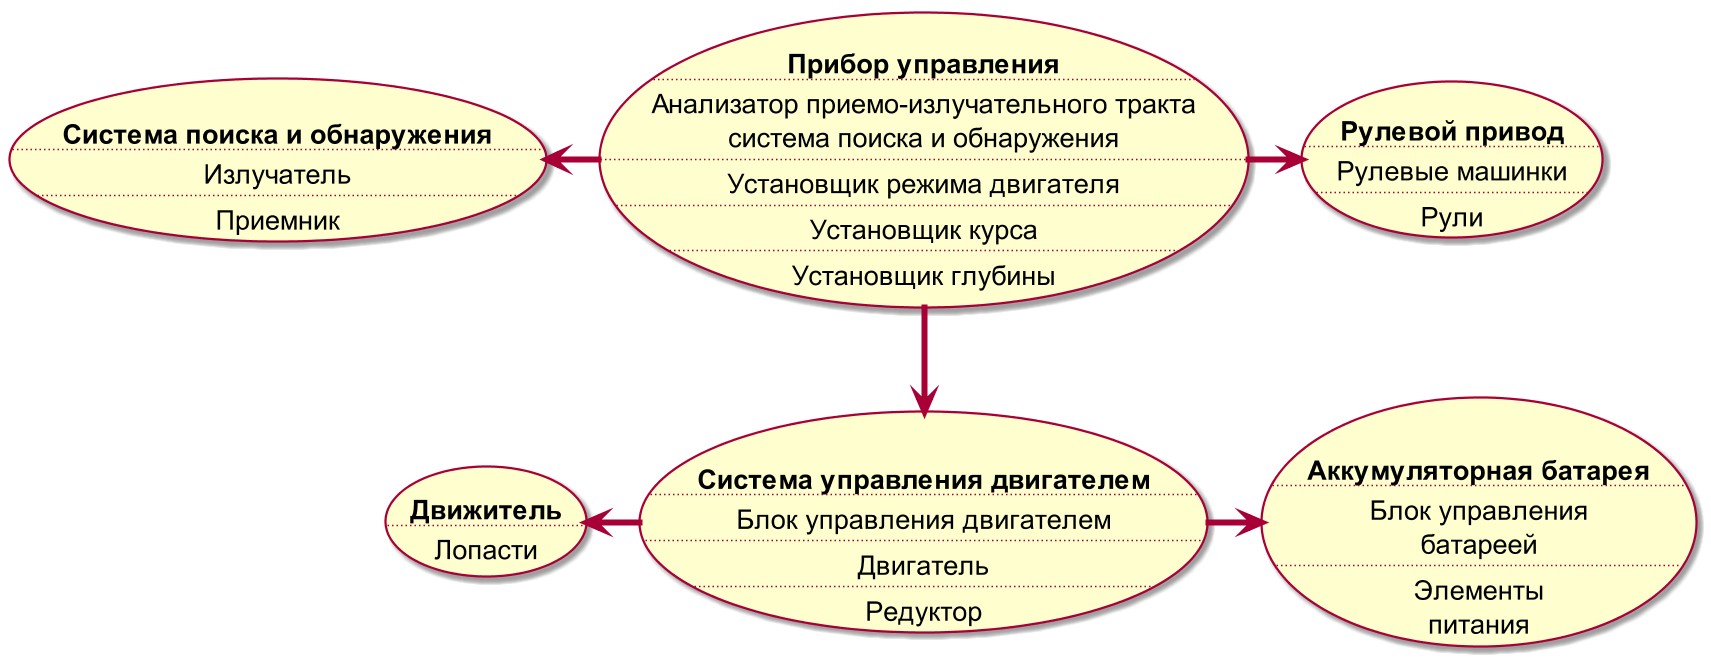
\includegraphics[width=.9\textwidth,keepaspectratio]{model_anpa}
        \caption{Декомпозиция материальной составляющей АНПА на составные части.}
            \label{fig:model_anpa}
    \end{figure}
\end{center}
%
Так же выделим \textbf{функции--действия} АНПА, которые показаны в таблицах
\ref{tbl:model_anpa_informations}, \ref{tbl:model_anpa_actions} \cite{journal:vestnik_igeu:elizarova}.
%
\begin{landscape}
\begin{longtable}[c]{llm{.25\textwidth}||l|l|m{.25\textwidth}||llm{.25\textwidth}}
\caption{Декомпозиция организационной составляющей модели АНПА на \textbf{объекты}, \textbf{функции} и \textbf{действия}.}
\label{tbl:model_anpa_decompose}\\
\hline
\multicolumn{3}{|c||}{\textbf{Объекты}}                                                                                     & \multicolumn{3}{c||}{\textbf{Функции}}                                                                  & \multicolumn{3}{c|}{\textbf{Действия}}                                                                                                  \\ \hline
\endhead
%
\multicolumn{1}{|c|}{\textbf{1}}           & \multicolumn{1}{c|}{\textbf{2}} & \multicolumn{1}{c||}{\textbf{3}}            & \multicolumn{1}{c|}{\textbf{1}}   & \multicolumn{1}{c|}{\textbf{2}} & \multicolumn{1}{c||}{\textbf{3}} & \multicolumn{1}{c|}{\textbf{1}}           & \multicolumn{1}{c|}{\textbf{2}} & \multicolumn{1}{c|}{\textbf{3}}                           \\ \hline
\multicolumn{1}{|l|}{\multirow{2}{*}{СПО}} & \multicolumn{1}{l|}{1}          & Излучатель                                  & \multirow{5}{*}{Движение}         & 1                               & Вперед                           & \multicolumn{1}{l|}{\multirow{3}{*}{ПУ}}  & \multicolumn{1}{l|}{1}          & \multicolumn{1}{l|}{Пеленгация целей}                     \\ \cline{2-3} \cline{5-6} \cline{8-9} 
\multicolumn{1}{|l|}{}                     & \multicolumn{1}{l|}{2}          & Приемник                                    &                                   & 2                               & Вправо                           & \multicolumn{1}{l|}{}                     & \multicolumn{1}{l|}{2}          & \multicolumn{1}{l|}{Коррекция курса}                      \\ \cline{1-3} \cline{5-6} \cline{8-9} 
\multicolumn{1}{|l|}{\multirow{4}{*}{ПУ}}  & \multicolumn{1}{l|}{3}          & Анализатор приемо-излучательного тракта СПО &                                   & 3                               & Влево                            & \multicolumn{1}{l|}{}                     & \multicolumn{1}{l|}{3}          & \multicolumn{1}{l|}{Коррекция глубины}                    \\ \cline{2-3} \cline{5-9} 
\multicolumn{1}{|l|}{}                     & \multicolumn{1}{l|}{4}          & Установщик режима двигателя                 &                                   & 4                               & Вверх                            & \multicolumn{1}{l|}{\multirow{2}{*}{АКБ}} & \multicolumn{1}{l|}{4}          & \multicolumn{1}{l|}{Хранение электроэнергии}              \\ \cline{2-3} \cline{5-6} \cline{8-9} 
\multicolumn{1}{|l|}{}                     & \multicolumn{1}{l|}{5}          & Установщик курса                            &                                   & 5                               & Вниз                             & \multicolumn{1}{l|}{}                     & \multicolumn{1}{l|}{5}          & \multicolumn{1}{p{.25\textwidth}|}{Доставка электроэнергии потребителям} \\ \cline{2-9} 
\multicolumn{1}{|l|}{}                     & \multicolumn{1}{l|}{6}          & Установщик глубины                          & \multirow{5}{*}{Питание}          & 6                               & СПО                              & \multicolumn{1}{l|}{Д}                    & \multicolumn{1}{l|}{6}          & \multicolumn{1}{l|}{Толкает водную среду}                 \\ \cline{1-3} \cline{5-9} 
\multicolumn{1}{|l|}{\multirow{3}{*}{СУД}} & \multicolumn{1}{l|}{7}          & БУД                                         &                                   & 7                               & ПУ                               &                                           &                                 &                                                           \\ \cline{2-3} \cline{5-6}
\multicolumn{1}{|l|}{}                     & \multicolumn{1}{l|}{8}          & Двигатель                                   &                                   & 8                               & СУД                              &                                           &                                 &                                                           \\ \cline{2-3} \cline{5-6}
\multicolumn{1}{|l|}{}                     & \multicolumn{1}{l|}{9}          & Редуктор                                    &                                   & 9                               & РП                               &                                           &                                 &                                                           \\ \cline{1-3} \cline{5-6}
\multicolumn{1}{|l|}{\multirow{2}{*}{РП}}  & \multicolumn{1}{l|}{10}         & РМ                                          &                                   & 10                              & Д                                &                                           &                                 &                                                           \\ \cline{2-6}
\multicolumn{1}{|l|}{}                     & \multicolumn{1}{l|}{11}         & Рули                                        & \multirow{2}{*}{Обнаружение}      & 11                              & Излучение зондирующей посылки    &                                           &                                 &                                                           \\ \cline{1-3} \cline{5-6}
\multicolumn{1}{|l|}{Д}                    & \multicolumn{1}{l|}{12}         & Лопасти                                     &                                   & 12                              & Прием отраженого сигнала         &                                           &                                 &                                                           \\ \cline{1-6}
\multicolumn{1}{|l|}{\multirow{2}{*}{АКБ}} & \multicolumn{1}{l|}{13}         & БУБ                                         & \multirow{4}{*}{Принятие решений} & 13                              & Изменить скорость движения       &                                           &                                 &                                                           \\ \cline{2-3} \cline{5-6}
\multicolumn{1}{|l|}{}                     & \multicolumn{1}{l|}{14}         & Модули питания                              &                                   & 14                              & Изменить курс                    &                                           &                                 &                                                           \\ \cline{1-3} \cline{5-6}
                                           &                                 &                                             &                                   & 15                              & Изменить глубину хода            &                                           &                                 &                                                           \\ \cline{5-6}
                                           &                                 &                                             &                                   & 16                              & Изменить тип зондирующей посылки &                                           &                                 &                                                           \\ \cline{4-6}
\end{longtable}
\end{landscape}
%
Исходя из данных, представленных в таблицах \ref{tbl:model_anpa_objects}, \ref{tbl:model_anpa_informations}, \ref{tbl:model_anpa_actions}
строятся матрицы $A, B$.
Взаимосвязь \textbf{объектов} и \textbf{функций} представляется матрицей $A$,
а \textbf{функций} и \textbf{действий} --- матрицей $B$:
%
\begin{equation}
    A = \begin{pmatrix}
        0 & 0 & 0 & 0 & 0 & 1 & 0 & 0 & 0 & 0 &1 & 0 & 0 & 0 & 0 & 0 \\
        0 & 0 & 0 & 0 & 0 & 1 & 0 & 0 & 0 & 0 & 0 & 1 & 0 & 0 & 0 & 0 \\
        0 & 0 & 0 & 0 & 0 & 1 & 1 & 0 & 0 & 0 & 0 & 1 & 0 & 0 & 0 & 1 \\
        0 & 0 & 0 & 0 & 0 & 0 & 0 & 1 & 0 & 1 & 0 & 0 & 0 & 0 & 0 & 0 \\
        0 & 1 & 1 & 0 & 0 & 0 & 0 & 0 & 0 & 0 & 1 & 0 & 0 & 1 & 0 & 1 \\
        0 & 0 & 0 & 1 & 1 & 0 & 0 & 0 & 0 & 0 & 0 & 0 & 0 & 0 & 1 & 0 \\
        0 & 0 & 0 & 0 & 0 & 1 & 0 & 0 & 0 & 0 & 0 & 0 & 1 & 0 & 0 & 0 \\
        0 & 0 & 0 & 0 & 0 & 1 & 0 & 0 & 0 & 0 & 0 & 0 & 1 & 0 & 0 & 0 \\
        0 & 0 & 0 & 0 & 0 & 0 & 0 & 0 & 0 & 1 & 0 & 0 & 0 & 0 & 0 & 0 \\
        1 & 1 & 1 & 1 & 1 & 0 & 0 & 0 & 0 & 0 & 0 & 0 & 0 & 1 & 1 & 0 \\
        1 & 1 & 1 & 1 & 1 & 0 & 0 & 0 & 0 & 0 & 0 & 0 & 0 & 1 & 1 & 0 \\
        0 & 0 & 0 & 0 & 0 & 0 & 0 & 0 & 0 & 0 & 0 & 0 & 0 & 1 & 1 & 0 \\
        0 & 0 & 0 & 0 & 0 & 1 & 1 & 1 & 1 & 1 & 1 & 0 & 0 & 0 & 0 & 0 \\
        0 & 0 & 0 & 0 & 0 & 0 & 0 & 0 & 0 & 0 & 1 & 1 & 0 & 0 & 0 & 0 \\
    \end{pmatrix},
%
    B = \begin{pmatrix}
        0 & 0 & 0 & 0 & 0 & 1 \\
        0 & 1 & 0 & 0 & 0 & 0 \\
        0 & 1 & 0 & 0 & 0 & 0 \\
        0 & 0 & 1 & 0 & 0 & 0 \\
        0 & 0 & 1 & 0 & 0 & 0 \\
        0 & 0 & 0 & 1 & 1 & 0 \\
        0 & 0 & 0 & 1 & 1 & 0 \\
        0 & 0 & 0 & 1 & 1 & 0 \\
        0 & 0 & 0 & 1 & 1 & 0 \\
        0 & 0 & 0 & 1 & 1 & 0 \\
        1 & 0 & 0 & 0 & 1 & 0 \\
        1 & 1 & 0 & 0 & 0 & 0 \\
        0 & 1 & 1 & 0 & 0 & 1 \\
        0 & 1 & 0 & 0 & 0 & 1 \\
        0 & 0 & 1 & 0 & 0 & 1 \\
        1 & 0 & 0 & 0 & 1 & 0 \\
    \end{pmatrix}\,.
\end{equation}

Ненулевое значение элемента матрицы $a_{ij}$ означает, что есть соответствие между материальным объектом $i$ и функцией $j$.
Например, $a_{11,\,14} = 1$ означает что объект \textit{рули} имеет функции \textit{изменение курса}.
Аналогично $b_{ij} \ne 0$ обозначает наличие ассоциации между функцией $i$ и действием $j$.
Например, $b_{13,\,3} = 1$ соответствует действию \textit{коррекция глубины} и связана с функцией \textit{изменить скорость движения}.

В результате умножения матриц $A$ и $B$ получаем матрицу $C_1$ размера $(6\times14)$,
которая определяет использование сущностей материальной составляющей предметной области действий, найденных через функции:

\begin{equation}
    C_1 = A \times B = \begin{pmatrix}
        1 & 0 & 0 & 1 & 2 & 0 \\
        1 & 1 & 0 & 1 & 1 & 0 \\
        2 & 1 & 0 & 2 & 3 & 0 \\
        0 & 0 & 0 & 2 & 2 & 0 \\
        2 & 3 & 0 & 0 & 2 & 1 \\
        0 & 0 & 3 & 0 & 0 & 1 \\
        0 & 1 & 1 & 1 & 1 & 1 \\
        0 & 1 & 1 & 1 & 1 & 1 \\
        0 & 0 & 0 & 1 & 1 & 0 \\
        0 & 3 & 3 & 0 & 0 & 3 \\
        0 & 3 & 3 & 0 & 0 & 3 \\
        0 & 1 & 1 & 0 & 0 & 2 \\
        1 & 0 & 0 & 5 & 6 & 0 \\
        2 & 1 & 0 & 0 & 1 & 0 \\
    \end{pmatrix}.
\end{equation}

Если $c_{1ik} = 0$, то сущность с номером $i$ не используется в функции с номером $k$ данной функции,
а если $c_{1ik} \ne 0$, то используется.

Построчное суммирование элементов матрицы $C_1$ получаем матрицу $C_2$, показывающую количественные характеристики
использования сущностей материальной составляющей предметной области в функциях:

\begin{equation*}
    C_2 = \begin{pmatrix}
        \sum_{j=1}^l c_{11j} \\
        \ldots \\
        \sum_{j=1}^l c_{1mj} \\
    \end{pmatrix} 
    =
    \begin{pmatrix}
        4 \\
        4 \\
        8 \\
        4 \\
        8 \\
        4 \\
        5 \\
        5 \\
        2 \\
        9 \\
        9 \\
        4 \\
        12 \\
        4 \\
    \end{pmatrix}.
\end{equation*}
где $c_{2i}$ количество функций, в которых используется данная сущность.

Делением матрицы $C_2$ на число $l = 6$, равное количеству действий в функциональной модели, получаем матрицу $C_3$,
содержащую относительные коэффициенты использования сущностей в действиях:
\begin{equation}
    C_3 = C_2 / l = \begin{pmatrix}
        0,67 \\
        0,67 \\
        \textbf{1,33} \\
        0,67 \\
        \textbf{1,33} \\
        0,67 \\
        0,83 \\
        0,83 \\
        0,33 \\
        \textbf{1,50} \\
        \textbf{1,50} \\
        0,67 \\
        \textbf{2,00} \\
        0,67 \\
    \end{pmatrix}.
\end{equation}
Установив пороговое значение $K_{min} = \overline{C_3} = 0.98$ получаем, что общесистемными являются
\textit{блок управления батареей (2.0);
    рулевые машинки, рулевой привод (1.5);
    анализатор приемо-излучательного тракта СПО и установщик курса (1.33)}.

Эти общесистемные объекты должны быть реализованы в имитационной модели в первую очередь.
Проведем более детальное рассмотрение этих объектов и информационных пакетов присущих им.


\subsection{Обоснование типов имитируемых сигналов}

\subsubsection{Имитация внешнего окружения}\label{sec:model_anpa:outer_params}
Ко внешним параметрам среды в рассматриваемой модели относится
глубина хода АНПА, эхо-сигнал в ответ на зондирующую посылку,
поступающий на \textit{приемник} и обрабатываемый \textit{анализатором приемо-излучающего тракта} АНПА.

Значение глубины меняется в пределах $h \in [0, h_{max}]$, где $h_{max}$ -- максимально допустимая глубина погружения АНПА.
АНПА должен следовать на заданной глубине, обусловленной внутренними алгоритмами объекта контроля.
Контроль глубины осуществляется с помощью гидравлической системы,
показания с которой считываются аналоговым датчиком глубины и преобразуются АЦП в цифровой сигнал.
В общем случае гидравлическая система управляется системой контроля,
по заранее определенному алгоритму, соответствующему выбранному режиму проверки.

Таким образом имитация глубины хода АНПА производится по заданному сценарию
при выполнения условий, например, наличие тока потребления
и на произвольный набор моментов времени $\{t_1, t_2, \ldots, t_n\}$
происходит изменение глубины $\{h_1, h_2, \ldots, h_n\}$, соответственно.


Предполагается, что ПУ формирует управляющую команду $s_j$ испускаемого сигнала на внутренней шине данных,
которому ставится в соответствие множество допустимых ответов $s_j \Rightarrow \{r_j\} = \{r_{j1}, r_{j2}, \ldots, r_{jn}\}$.
В процессе имитации работы подменяются ответы $r_{ji}$.

Управляющая последовательность бит $s_j$, физически представляющая цифровой сигнал напряжением $|U_{\longrightarrow}|$.
Ответная последовательность бит $r_j$, напряжением $|U_{\longleftarrow}| < |U_{\longrightarrow}|$:
СК анализирует правильность ответа $r_j$ на воздействие $s_j$,
также анализируется величина тока, при $I_{\longleftarrow} \geq I_{min}$ биты в ответе $r_j$ считаются равными логической единице.
Цикл команд $s_j \Rightarrow r_j$ продолжается до конца выполнения выбранной задачи или до досрочной остановки.

Невыполнение заданной управляющей команды $s_j$ в течении заданного времени $t_{\mbox{max}}$,
подсистемы СПО АНПА считается аварийным.

Выдача определенного слова должна происходить при выполнении конечного множества условий как с задержкой, так и без нее.


\subsubsection{Имитация внутренних параметров АНПА}\label{sec:model_anpa:inner_params}
\textbf{Напряжение от АКБ.}
Информация о напряжениях \textit{модулей питания} АКБ $U_k, k\in [1..N]$ представляется вещественным числом,
для каждого модуля определяется допустимый диапазон напряжений $U_k \in [U_k^{min}, U_k^{max}]$,
выход за пределы которого считается аварийным и функционирование АНПА не допускается.

\textbf{Ток потребления абонентами АНПА.}
Суммарный ток потребления в имитационной модели определяется как $I_\Sigma = \sum_k I_k + \hat I$,
где токи контролируемых $N$ узлов системы $I_k,\, k\in[1..N]$ и $\hat I$ --- ток узлов не подлежащих контролю (не описанные в модели или флуктуации),
являются аналоговыми реакциями. % $A^r_{out}$.

Допустимый диапазон изменений токов $k$-го узла $I_k \in [I_k^{min}, I_k^{max}]$ обусловлен электрической схемой бортовой сети АНПА.
Аналогично $\hat I \in [\hat I^{min}, \hat I^{max}]$ находится в неком диапазоне.
Следовательно суммарный ток потребления АНПА также имеет некое распределение $I_\Sigma \in [I_\Sigma^{min}, I_\Sigma^{max}]$.
Выход одного параметров из допустимого диапазона $I_\Sigma, I_k, \hat I$ считается аварийным режимом работы АНПА.

Выдача определенного напряжения и тока должны происходить при выполнении определенных условий,
например, таких как инициализация некой заданной программы работы АНПА, которая
отождествляется с набором управляющих воздействий и ответных реакций на них.
Также значение $I_\Sigma$ может меняться в процессе проверки, для модулирования включения или выключений узлов,
то есть в общем случае может быть набор $I_\Sigma^{\langle k \rangle}$ для $k$-го состояния АНПА.
Таким образом, достаточно следить за конечным набором параметров и
имитировать напряжения и токи моментально или с некой задержкой $\tau$.

\textbf{Работа СУД.}
Согласно выбранной программе проверки на СК вырабатывается соответствующая 
частота $f$ вращения вала \textit{двигателя} в виде ШИМ сигнала.
Из АНПА возвращается периодический сигнал о прохождении определенной дистанции (метка кратного прохождения $m$ метров).
Выход периода $T \in [T^{min}, T^{max}]$ или скважности $Q \in [Q^{min}, Q^{max}]$ из допустимых диапазонов
СК рассматривается как аварийный режим.

ПУ обменивается целочисленными управляющими командами в формате запрос-ответ с СУД по шине данных, в частности с БУД,
для установки необходимого режима работы \textit{двигателя}.

Таким образом имитация вращения валов винтов производится выработкой прямоугольного сигнала с заданным периодом $T$ и скважностью $Q$,
аналогично --- имитация генерации АНПА метки $m$ пройденной дистанции
(увеличение контролируемого параметра на заданную величину $\delta \in \mathcal{R}$ с периодичностью $T_m$ в течении времени $\tau$).

\textbf{Работа рулевой системы.}
ПУ устанавливает заданные курс и глубину в следствии чего подсистема РП
осуществляет перекладку рулей, по средствам \textit{рулевых машинок}.
Информация с РМ может быть получена различными способами, в зависимости от их конструктивного исполнения.
Это может быть напряжение с потенциометров обратной связи, которое обрабатывается в БГР системы контроля
и передается в виде преобразованного цифрового сигнала
либо это может быть изначально  цифровой сигнал.

При проектировании АНПА устанавливается соответствие между $\langle s_j, \{r_j\} \rangle \Rightarrow \omega_i = \omega_i(s_j, \{r_j\}), i\in [1..N]$,
где $s_j, r_j$ -- управляющие и ответные последовательности из раздела \ref{sec:model_anpa:outer_params},
$\omega_i$ -- заданные перекладки рулей для $N$ рулевых машинок.
Если на воздействие $s_j$ приходит ответ $r_{ji} \in \{r_j\}$, в котором содержится информация о том что,
поисковая цель находится по курсу $\bar \omega$, то должны быть установлены соответствующие значения перекладок рулей,
которые приведут к изменению курса (и/или глубины) для оптимального достижения поисковой цели.


\subsection*{Выводы}
Принимая во внимание результаты анализа взаимосвязей составных частей АНПА,
имитационная модель АНПА строится на основе следующих компонентов:
\begin{itemize}
    \item непосредственная запись значения при выполнении единичного условия;
    \item отложенная запись значения при выполнении единичного условия;
    \item непосредственная запись значения при выполнении множественных условий;
    \item отложенная запись значения при выполнении множественных условий;
    \item периодическое изменение на заданную величину в течении определенного времени.
\end{itemize}

В АНПА в общем случае может быть множество шин данных, по которым происходит обмен между СЧ АНПА и системой контроля.
СК в свою очередь так же может использовать набор протоколов для обмена информацией с АНПА
или для обработки первичного набора сигналов от АНПА.
Одним из таких интерфейсов является Modbus, так как после прохождения первичных сигналов через БГР
они поступают на ПЛК, который взаимодействует с ПО верхнего уровня, например, по протоколу Modbus~TCP/IP.
Далее будет показана модель \textit{решающая} задачу имитации взаимодействия СК с АНПА.
